\documentclass{mynotes}


\title{Notes on the prelimit patterns in synchronized asymmetrically coupled van der Pol oscillators }

\author[1]{ Tony Savostianov}
\author[2]{ Sasha Shapoval }
\author[3]{ Mikhail Shnirman}

\affil[1]{ Computational Network Science, RWTH Aachen   \\ \mbox{email: \email{savostianov@cs.rwth-aachen.de}} }
\affil[2]{  University of Lodz, Department of Mathematics and Computer Science, \L{}\'od\.z, Poland  \mbox{email: \email{alexander.shapoval@wmii.uni.lodz.pl} }}
\affil[3]{ Institute of Earthquake Prediction Theory and Mathematical Geophysics RAS, Moscow, Russia }

\keywords{ coupled oscillators }

\usepackage{tikz-network}
\usepackage{faktor}
\usepackage{comment}

\usepackage{algorithm}% http://ctan.org/pkg/algorithms
\usepackage{algpseudocode}
\graphicspath{./figures/}

\usepackage{tikz}
\usepackage{pgfplots}

\usetikzlibrary{arrows.meta}
\usetikzlibrary{backgrounds}
\usepgfplotslibrary{patchplots}
\usepgfplotslibrary{fillbetween}
\pgfplotsset{%
     layers/standard/.define layer set={%
         background,axis background,axis grid,axis ticks,axis lines,axis tick labels,pre main,main,axis descriptions,axis foreground%
     }{
         grid style={/pgfplots/on layer=axis grid},%
         tick style={/pgfplots/on layer=axis ticks},%
         axis line style={/pgfplots/on layer=axis lines},%
         label style={/pgfplots/on layer=axis descriptions},%
         legend style={/pgfplots/on layer=axis descriptions},%
         title style={/pgfplots/on layer=axis descriptions},%
         colorbar style={/pgfplots/on layer=axis descriptions},%
         ticklabel style={/pgfplots/on layer=axis tick labels},%
         axis background@ style={/pgfplots/on layer=axis background},%
         3d box foreground style={/pgfplots/on layer=axis foreground},%
     },
 }

 \usetikzlibrary{decorations.pathreplacing,decorations.markings}
 \tikzset{
   % style to apply some styles to each segment of a path
   on each segment/.style={
     decorate,
     decoration={
       show path construction,
       moveto code={},
       lineto code={
         \path [#1]
         (\tikzinputsegmentfirst) -- (\tikzinputsegmentlast);
       },
       curveto code={
         \path [#1] (\tikzinputsegmentfirst)
         .. controls
         (\tikzinputsegmentsupporta) and (\tikzinputsegmentsupportb)
         ..
         (\tikzinputsegmentlast);
       },
       closepath code={
         \path [#1]
         (\tikzinputsegmentfirst) -- (\tikzinputsegmentlast);
       },
     },
   },
   % style to add an arrow in the middle of a path
   mid arrow/.style={postaction={decorate,decoration={
         markings,
         mark=at position .5 with {\arrow[#1]{stealth}}
       }}},
 }
 


%%%% COMMANDS %%%%%%%%%%%%%%%%%%%%%%%%

\newcommand*{\insidefigure}[3][0.5\columnwidth]{
      \begin{center}
            \begin{minipage}{#1}
                  \centering
                  #2
                  \captionof{figure}{#3}
            \end{minipage}
      \end{center}
}

\newcommand*{\mc}[1]{\mathcal{#1}}
\renewcommand*{\bar}[1]{\overline{#1}}
\renewcommand*{\b}[1]{\mathbf{#1}}
\newcommand*\eps{\varepsilon}
\newcommand*{\V}[1]{ \mc V_{#1}(\mc K)}
\newcommand*{\vn}{\varnothing}
\newcommand*{\ord}[1]{\mathrm{ord}\,(#1)}

\usepackage{dsfont}
\newcommand*{\ds}[1]{\mathds{#1}}

\newcommand*{\Lu}[1]{L_{#1}^{\uparrow}}
\newcommand*{\bLu}[1]{{\overline{L}^{\uparrow}}_{#1}}
\newcommand*{\Ld}[1]{L_{#1}^{\downarrow}}
\newcommand*{\bLd}[1]{{\overline{L}^{\downarrow}}_{#1}}

\newcommand*{\wh}[1]{\widehat{#1}}


\renewcommand*{\bar}[1]{ \overline{#1} }


\newcommand{\algname}{\texttt{HeCS}}


\DeclareMathOperator{\im}{im}
\let\span\relax
\DeclareMathOperator{\span}{span}
\DeclareMathOperator{\Sym}{Sym}
\DeclareMathOperator{\Tr}{Tr}

\DeclareMathOperator{\Corr}{\mathbf{Corr}}







\usetikzlibrary{patterns}
\definecolor{bananamania}{rgb}{0.98, 0.91, 0.71}
\definecolor{lavender}{rgb}{0.4470588235294118, 0.5294117647058824, 0.992156862745098}
\definecolor{burntsienna}{rgb}{0.91, 0.45, 0.32}
\definecolor{airforceblue}{rgb}{0.36, 0.54, 0.66}
\definecolor{liberty}{HTML}{5158BB}
\definecolor{junglegreen}{rgb}{0.16, 0.67, 0.53}
\definecolor{persimmon}{HTML}{DE5A02}


\newcommand{\AxisRotator}[1][rotate=0]{%
    \tikz [x=0.15cm,y=0.15cm,line width=.2ex,-stealth,#1] \draw (0,0) arc (-150:150:1 and 1);%
}
\newcommand{\AxisRotatorMirror}[1][rotate=0]{%
    \tikz [x=0.15cm,y=0.15cm,line width=.2ex,-stealth,#1] \draw (0,0) arc (150:-150:1 and 1);%
}
\newcommand{\EVert}[2]{%
\left[\begin{smallmatrix} #1 \\ #2 \end{smallmatrix}\right]
}
\newcommand{\TVert}[3]{%
\left[\begin{smallmatrix} #1 \\ #2 \\ #3 \end{smallmatrix}\right]
}

\usepackage{amsthm}
\usepackage[capitalize, nameinlink]{cleveref}
\crefdefaultlabelformat{\color{liberty}#1#2#3}


\crefname{section}{section}{sections}
\crefname{subsection}{subsection}{subsections}
\Crefname{section}{Section}{Sections}
\Crefname{subsection}{Subsection}{Subsections}
\Crefname{figure}{Figure}{Figures}
\Crefname{definition}{Definition}{Definitions}
\Crefname{proposition}{Proposition}{Propositions}
\Crefname{lemma}{Lemma}{Lemmas}
\Crefname{remark}{Remark}{Remarks}
\Crefname{problem}{Problem}{Problems}
\crefformat{equation}{\textup{#2(#1)#3}}
\crefrangeformat{equation}{\textup{#3(#1)#4--#5(#2)#6}}
\crefmultiformat{equation}{\textup{#2(#1)#3}}{ and \textup{#2(#1)#3}}
{, \textup{#2(#1)#3}}{, and \textup{#2(#1)#3}}
\crefrangemultiformat{equation}{\textup{#3(#1)#4--#5(#2)#6}}%
{ and \textup{#3(#1)#4--#5(#2)#6}}{, \textup{#3(#1)#4--#5(#2)#6}}{, and \textup{#3(#1)#4--#5(#2)#6}}

\Crefformat{equation}{#2Equation~\textup{(#1)}#3}
\Crefrangeformat{equation}{Equations~\textup{#3(#1)#4--#5(#2)#6}}
\Crefmultiformat{equation}{Equations~\textup{#2(#1)#3}}{ and \textup{#2(#1)#3}}
{, \textup{#2(#1)#3}}{, and \textup{#2(#1)#3}}
\Crefrangemultiformat{equation}{Equations~\textup{#3(#1)#4--#5(#2)#6}}%
{ and \textup{#3(#1)#4--#5(#2)#6}}{, \textup{#3(#1)#4--#5(#2)#6}}{, and \textup{#3(#1)#4--#5(#2)#6}}

\crefdefaultlabelformat{#2\textup{#1}#3}




%\newcommand{\algname}{\texttt{HeCS}}


\newtheorem{problem}{Problem}

\usepackage{enumitem}

\DeclareMathOperator{\diag}{diag} 

\newenvironment{mt}{\begin{pmatrix}}{\end{pmatrix}}

\usepackage{multirow}
\usepackage{booktabs}

\usepackage{nicematrix}

\NiceMatrixOptions
  {
    custom-line = 
     {
       letter = : ,
       command = dashedline , 
       ccommand = cdashedline ,
       tikz = dotted
     }
  }

  \setcounter{MaxMatrixCols}{20}
  \usepackage{amsmath}
  \allowdisplaybreaks
  
\usepackage{wasysym}
\usepackage{stackengine}

\makeatletter
\newcommand*\bigcdot{\mathpalette\bigcdot@{.5}}
\newcommand*\bigcdot@[2]{\mathbin{\vcenter{\hbox{\scalebox{#2}{$\m@th#1\bullet$}}}}}
\makeatother

  \newcommand\obullet[1]{\ensurestackMath{\stackon[0pt]{#1}{\mkern1mu\bigcdot}}}
%\renewcommand{\dot}{\obullet}

\DeclareMathOperator*{\vect}{\mathrm{diagvec}}
\DeclareMathOperator*{\grad}{\mathrm{grad}}
\DeclareMathOperator*{\diver}{\mathrm{div}}
\DeclareMathOperator*{\curl}{\mathrm{curl}}

\newcommand\mr{\min^+_{\mathrm{row}}}
\renewcommand*{\deg}{\mathrm{deg}}
\newcommand\scal[1]{\left\langle {#1} \right\rangle}

%\usepackage[caption=false]{subfig}

\DeclareMathOperator*{\argmin}{arg\,min}
\DeclareMathOperator*{\argmax}{arg\,max}
\usepackage{xfrac}

%\usepackage{unicode-math}
%\usepackage{fontspec}

%\setmainfont{Zed Sans Light Extended}
%\setmainfont{Nunito Light}
%\setmainfont{Poppins Light}
%\setmathfont{Iwona Light}
%\setmathfont[Scale=1.5]{Nunito Light}%\setmathfont[Scale=1.2]


\newcommand*{\dw}{\Delta\omega}

\begin{document}

\maketitle




\section{ Introduction }

Well, it would be nice to have one. 

You know, somewhere here, maybe\dots

\paragraph*{ Related works. }


\paragraph*{ Contributions. } we \emph{do} contribute something, right?
\paragraph*{ Outline. } it's all over the place\dots






\section{ Model }

We consider the space-time normalized model of two dissipatively coupled van der Pol (vdP) oscillators given by:
\begin{equation} \label{eq:system}
    \begin{aligned}
        & \ddot x  - ( 1 - x^2 ) \dot x + ( 1 - \dw ) x + \mu_1 ( \dot x - \dot y ) = 0       \\
        &  \ddot y  - ( 1 - y^2 ) \dot y + ( 1 + \dw ) y + \mu_2 ( \dot y - \dot x ) = 0  
    \end{aligned},
\end{equation}
where \( 0 < \dw < 1 \) is a \emph{ normalized relative frequency difference } and \( \mu_i \le 0 \) describe couplings\todo{in case it might be useful, lets set \(  \mu_1 + \mu_2 = 2 \mu \) and \( | \mu_1 - \mu_2 | = 2 \Delta \mu \)}. Note that \( x \) is set to be a ``faster'' of two oscillators and one should consider different setups in terms of which oscillator (the ``fast'' one or the ``slow'' one ) has larger coupling.

Notable cases:
\begin{itemize}[itemsep = -0.25em, topsep = -0.5em]
      \item[(i)] \emph{ symmetric coupling }, \( \mu_1 = \mu_2 \), previously studied and should be used as reference point; 
      \item[(ii)] \emph{fancy RHS}, e.g. \( \mu_2 = 0 \), so 
      \begin{equation}
            \begin{aligned}
                  & \ddot x  - ( 1 - \mu_1 - x^2 ) \dot x + ( 1 - \dw ) x = \mu_1 \dot y     \\
                  &  \ddot y  - ( 1 - y^2 ) \dot y + ( 1 + \dw ) y   = 0  
              \end{aligned} 
      \end{equation}
      which mimic a case of vdP with a ``resonant'' RHS\todo{it is not really a resonance, since the amplitude on the right correspond to some function a frequency on the left, but \emph{maybe}\dots}.
\end{itemize}

\begin{remark}[Half-sum/half-diff notation]
      On par with the previous papers, we provide the same dynamics as in \Cref{eq:system} under the following change of variables:
      \begin{equation}
            \begin{cases}
                  2u = x + y \\
                  2v = x - y 
            \end{cases}
            \qquad 
            \begin{cases}
                  x = u + v \\
                  y = u - v
            \end{cases},
      \end{equation}
      so we obtain
      \begin{equation}
            \label{eq:uv}
            \begin{aligned}
                  & \ddot u - ( 1 - u^2 - v^2 ) \dot u + u - \dw v + 2 u v \dot v + \textcolor{rwth-red}{ 2 \Delta\mu \dot v  } = 0 \\
                  & \ddot v - ( 1 - u^2 - v^2 ) \dot v + v - \dw u + 2 v u \dot u + 2 \mu \dot v = 0 
            \end{aligned}
      \end{equation}
      with the highlighted term concentrates the asymmetry of the coupling.
\end{remark}

\section{ Synchronization }

All of our consideration and defined entities are well-posed only for synchronized pair of oscillators. Specifically, one normally distinguishes two types of synchronization, in \emph{ frequency } and \emph{ phase }. Recall that in the case of symmetric coupling \( \mu_1 = \mu_2 \), the synchronization seemed to be joint, i.e. frequency synchronization necessarily implied phase synchronization and vice versa\todo{it is worth revisiting it around the threshold, we haven't properly tested it in the ``battle'' region}.

\begin{remark}[Synchronization inequality from simpler times]\label{rem:kuramoto_synch}
      Under specific simplifying assumptions, one may reduce symmetrically coupled vdP system ( \Cref{eq:system} ) to a simple Kuramoto model where the synchronization is achieved if and only if \( \mu > \dw \); previously, we inherited that property for the symmetric vdP system which seeemed to hold experimentally.
      \\[5pt]

      At the same time, in the nonsymmetric Kuramoto case, assuming initial frequencies \( \Omega_1 \) and \( \Omega_2 \), the system is synchronized if \[ \mu_1 > \Omega_1 - \Omega_0  \text{ and } \mu_2 > \Omega_2 - \Omega_0 \] where \( \Omega_0 \) is the common synchronized frequency, \( \Omega_0 = \frac{ \mu_1 \Omega_1 + \mu_2 \Omega_2 }{ \mu_1 + \mu_2 } \). Note that this principle may be expected to largely translate to the vdP case with certain caveats; specifically, it is challenging to redefine \( \Omega_0 \) since even for \( \mu_1 = \mu_2 = \mu \) the common frequency was shown to be dependent on \( \mu \), \( \Omega_0 = \Omega_0 ( \mu ) \), albeit this dependence is rather small.
\end{remark}
\todo{probably worth recalling some series expansions here}.


\subsection{Barcode diagrams}

Here we formulate a straightforward method to test the synchronization of two oscillators, \Cref{eq:system}. 

We base our estimates on the relative placement of local minima of \( \{ x(t), y(t) \} \); namely,
\begin{enumerate}[ topsep = -0.5em, itemsep = -0.25em ]
      \item[\color{rwth-blue}(i)] solve the system (\eqref{eq:system}) for long-enough time (specifically, we solve for \( [ 0; T ] = [ 0; 2 \pi N ]\), \( N = 100 \) ); this length is based on the notion that the first order approximation of the isolated vdP frequency is \( 1 \), so the first order period is \( 2 \pi \) \todo{ here a reference for the series decomposition should be };
      \item[\color{rwth-blue}(ii)] for each oscillator \( \{ x(t), y(t) \} \) we extract position of local minima \( \{ \tau_x^{(i)} \}\) and \( \{ \tau_y^{(i)} \}\)  \todo{one can do this with preexisting tools, but the fact is that ODEsolver computes an approximation of \( \dot x \) and \( \dot y \), so one can extract minima from them};
      \item[\color{rwth-blue}(iii)] then one can define \textit{empirical} frequencies as \( \left\{ \Omega_x^{(i)} \right\} = \left\{ \frac{1}{ \tau_x^{(i+1)} - \tau_x^{(i)} } \right\} \) and \( \left\{ \Omega_y^{(i)} \right\} = \left\{ \frac{1}{ \tau_y^{(i+1)} - \tau_y^{(i)} } \right\} \) respectively; we measure the standard deviation of the frequency sequences \( \left\{ \Omega_x^{(i)} \right\} \) over the last \( 20 \) minima (relative to the mean value) to ascertain synchronization;
      \item[\color{rwth-blue}(iv)] finally, we posit that the phase difference \( \Delta\varphi \) never exceeds half a period, so in order to calculate it, we find for each minimum \( \tau_x^{(i)} \) the closest minimum \( \tau_y^{(j)} \); then, we say that \( \Delta\phi^{(i)} = \left| \tau_x^{(i)} - \tau_y^{(j)} \right| \) and compute the stability of the sequence in the same manner. 
\end{enumerate}
 
\begin{figure}[hbtp]
      \centering
      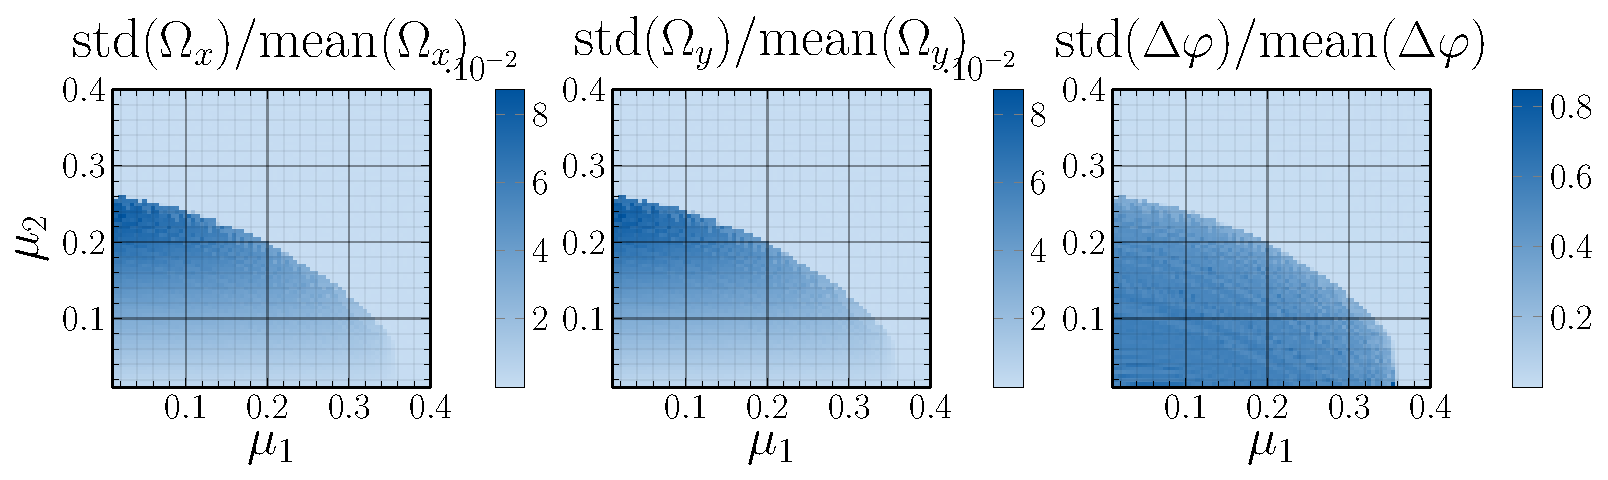
\includegraphics[width = 1.0\columnwidth]{figures/synch_heatmap.pdf}
      \caption{
            Synchronization of oscillators (\Cref{eq:system}) in frequency (left and center panes) and in phase (right pane). \( \dw = 0.2 \), integration time is set to \( N = 100 \).
            \label{fig:synch_heatmap}
      }
\end{figure}

We provide the stabilization of frequency and the phase difference in \Cref{fig:synch_heatmap}. It is worth pointing out that:
\begin{itemize}[ topsep = -0.5em, itemsep = -0.25em ]
      \item point \( \mu_1 = \mu_2 = \dw \) lends on the boundary, upholding observed behaviour in the symmetric case;
      \item in the case of \( \mu_1 = 0 \), Kuramoto synchronization (see \Cref{rem:kuramoto_synch}) requires \( \mu_2 \ge \dw \) (and vice versa), which is evidently too restrictive for the vdP case;
      \item phase and frequency synchronizations remain joint and are achieved simultaneously;
      \item the boundary is impressively pronounced, so one may at least attempt to speculate about the actual function and synchronization inequality.
\end{itemize}










\clearpage
%% BIBLIOGRAPHY %% 
\nocite{*}
\bibliographystyle{alpha}
\bibliography{notes}

\end{document}